\subsection{Approximation Methods}

\begin{figure}[H]
  \centering
  \begin{tikzpicture}[
  >=Stealth,
  x=4.8cm,
  y=1.75cm,
  every node/.style={font=\scriptsize},
  axis/.style={->, gray!70, line width=0.45pt},
  curve/.style={blue!70!black, line width=0.9pt},
  coarse/.style={orange!82!black, line width=0.75pt},
  fine/.style={teal!70!black, line width=0.65pt},
  point/.style={circle, fill=black, inner sep=1.05pt},
  note/.style={fill=white, inner sep=0.8pt}
]
  \draw[axis] (-0.04,0) -- (1.06,0) node[right] {$x$};
  \draw[axis] (0,-0.06) -- (0,1.08) node[above] {$y$};

  \draw[curve, domain=0:1, variable=\x, samples=140]
    plot (\x,{sqrt(1-\x)});
  \draw[coarse] (0,1) -- (0.5,0.7071) -- (1,0);
  \draw[fine] (0,1) -- (0.125,0.9354) -- (0.25,0.8660) -- (0.375,0.7906)
    -- (0.5,0.7071) -- (0.625,0.6124) -- (0.75,0.5) -- (0.875,0.3536) -- (1,0);

  \foreach \x/\y in {0/1,0.5/0.7071,1/0} {
    \node[point] at (\x,\y) {};
  }

  \node[blue!70!black, note] at (0.30,0.93) {$f$};
  \node[orange!82!black, note] at (0.64,0.56) {$P_2$};
  \node[teal!70!black, note] at (0.82,0.42) {$P_8$};
  \node[below] at (0,0) {$0$};
  \node[below] at (1,0) {$1$};
\end{tikzpicture}

  \caption{Finer piecewise-linear interpolants approach $f(x)=\sqrt{1-x}$ uniformly on $[0,1]$.}
  \label{fig:polygonal-approximation-sqrt-one-minus-x}
\end{figure}

\begin{theorem} \label{thm:weierstrass-polynomial-approximation}\label{thm:power-approx-fourier-main-source-todo} \hlt{Weierstrass Polynomial Approximation}\\
Let $a<b$ and $f\in C([a,b],\C)$. Then $\exists (P_n)\subset\C[x]$ with $P_n\rightrightarrows f$ on $[a,b]$. If $f([a,b])\subset\R$, choose $(P_n)\subset\R[x]$.
\begin{proof} By affine change and subtraction of the endpoint interpolant, reduce to $[0,1]$ with $f(0)=f(1)=0$.\\
Extend $f=0$ off $[0,1]$; then $f$ is uniformly continuous on $[-1,2]$. Choose $c_n>0$ so $Q_n(t)\defeq c_n(1-t^2)^n$ satisfies $\int_{-1}^{1}Q_n=1$. Use $c_n<\sqrt n$ and $Q_n(t)\leq\sqrt n(1-\delta^2)^n$ for $0<\delta\leq\abs{t}\leq1$. Set $P_n(x)\defeq\int_{-1}^{1}f(x+t)Q_n(t)\,dt$.\\
Since $P_n(x)=\int_0^1 f(u)Q_n(u-x)\,du$, $P_n\in\C[x]$, and $P_n\in\R[x]$ if $f$ is real-valued.\\
Given $\varepsilon>0$, choose $0<\delta\leq1$ with $\abs{u-v}<\delta\Rightarrow\abs{f(u)-f(v)}<\varepsilon/2$ on $[-1,2]$, and set $M=\sup_{[-1,2]}\abs{f}$.\\
For $x\in[0,1]$, $Q_n\geq0$, $\int_{-1}^{1}Q_n=1$ give $\abs{P_n(x)-f(x)}\leq\int_{-1}^{1}\abs{f(x+t)-f(x)}Q_n(t)\,dt\leq\frac{\varepsilon}{2}+4M\sqrt n(1-\delta^2)^n$.\\
Thus $\norm{P_n-f}_\infty\to0$ on $[0,1]$; undo the reductions.\\
\hlt{Structural Commentary}: Polynomial kernels approximate the identity.\\
\hlt{Key Insight}: Uniform continuity handles near mass; kernel concentration removes far mass.
\end{proof}
\end{theorem}

\begin{figure}[H]
  \centering
  \begin{tikzpicture}[
  >=Stealth,
  every node/.style={font=\scriptsize},
  x=2.55cm,
  y=0.88cm,
  axis/.style={->, black!55, line width=0.45pt},
  broad/.style={black!55, dashed, line width=0.75pt},
  narrow/.style={black!85, line width=0.9pt},
  window/.style={fill=gray!12, draw=none},
  guide/.style={black!35, dashed, line width=0.45pt}
]
  \draw[window] (-0.32,0) rectangle (0.32,2.75);

  \draw[axis] (-1.16,0) -- (1.16,0) node[right] {$t$};
  \draw[axis] (0,-0.15) -- (0,2.86);

  \draw[broad, domain=-1:1, samples=150]
    plot (\x,{1.25*(1-\x*\x)^2});
  \draw[narrow, domain=-1:1, samples=180]
    plot (\x,{2.48*(1-\x*\x)^8});

  \node at (0.66,0.88) {$Q_m$};
  \node at (0.34,1.75) {$Q_n$};

  \draw[guide] (-0.32,0) -- (-0.32,2.55);
  \draw[guide] (0.32,0) -- (0.32,2.55);
  \draw[<->, black!55] (-0.32,-0.22) -- node[below] {$2\delta$} (0.32,-0.22);

  \node[below] at (-1,0) {$-1$};
  \node[below] at (1,0) {$1$};
\end{tikzpicture}

  \caption{The normalized kernels $Q_n(t)=c_n(1-t^2)^n$ concentrate near $0$ while retaining integral $1$.}
  \label{fig:polynomial-bump-kernel}
\end{figure}

\begin{corollary} \label{cor:absolute-value-polynomial-approximation} \hlt{Polynomial Approximation of $\abs{x}$}\\
Let $a>0$. There exists $(P_n)\subset\R[x]$ such that $P_n(0)=0$ and $P_n\rightrightarrows\abs{x}$ on $[-a,a]$.
\begin{proof} By Theorem \ref{thm:weierstrass-polynomial-approximation}, choose $Q_n\in\R[x]$ with $Q_n\rightrightarrows\abs{x}$ on $[-a,a]$. Set $P_n(x)\defeq Q_n(x)-Q_n(0)$.\\
Then $P_n\in\R[x]$, $P_n(0)=0$, and $Q_n(0)\to0$, so $\norm{P_n-\abs{x}}_\infty\leq\norm{Q_n-\abs{x}}_\infty+\abs{Q_n(0)}\to0$.\\
\hlt{Structural Commentary}: Normalize at $0$.\\
\hlt{Key Insight}: The constant correction vanishes uniformly.
\end{proof}
\end{corollary}

\begin{definition} \label{def:algebra-uniform-closure-functions} \hlt{Algebras and Uniform Closure}\\
Let $\mathcal{A}$ be a family of complex-valued functions on a set $E$.
\begin{enumerate}[label=(\roman*)]
\setlength{\itemsep}{0pt}
\item $\mathcal{A}$ is an \hlt{algebra} if it is closed under $+$, products, and scalar multiplication (real scalars in the real case).
\item $\mathcal{A}$ is \hlt{uniformly closed} if $f_n\in\mathcal{A}$ and $f_n\rightrightarrows f$ on $E$ imply $f\in\mathcal{A}$.
\item The \hlt{uniform closure} of $\mathcal{A}$ is $\{f:f_n\in\mathcal{A},\ f_n\rightrightarrows f\text{ on }E\}$.
\end{enumerate}
\end{definition}

\begin{theorem} \label{thm:uniform-closure-algebra} \hlt{Uniform Closures Are Closed Algebras}\\
The uniform closure of an algebra of bounded functions is a uniformly closed algebra.
\begin{proof}
If $f,g\in\mathcal{B}$, choose $f_n,g_n\in\mathcal{A}$ with $f_n\rightrightarrows f$ and $g_n\rightrightarrows g$.\\
Boundedness and uniform convergence give $f_n+g_n\rightrightarrows f+g$; $f_ng_n\rightrightarrows fg$; and $cf_n\rightrightarrows cf$.
Thus $\mathcal{B}$ is an algebra. If $h_n\in\mathcal{B}$ and $h_n\rightrightarrows h$, approximate each $h_n$ uniformly by some $a_n\in\mathcal{A}$ within $1/n$; then $a_n\rightrightarrows h$, so $h\in\mathcal{B}$.\\
\hlt{Structural Commentary}: Uniform limits preserve algebraic operations for bounded functions.\\
\hlt{Key Insight}: The uniform closure of an algebra has already absorbed all further uniform limits.
\end{proof}
\end{theorem}

\begin{definition} \label{def:separates-points-vanishes-nowhere-self-adjoint} \hlt{Separation, Nonvanishing, and Self-Adjointness}\\
Let $\mathcal{A}$ be a family of functions on $E$.
\begin{enumerate}[label=(\roman*)]
\setlength{\itemsep}{0pt}
\item $\mathcal{A}$ \hlt{separates points} on $E$ if for every distinct $x_1,x_2\in E$ there is $f\in\mathcal{A}$ with $f(x_1)\neq f(x_2)$.
\item $\mathcal{A}$ \hlt{vanishes at no point} of $E$ if for every $x\in E$ there is $g\in\mathcal{A}$ with $g(x)\neq0$.
\item A complex algebra $\mathcal{A}$ is \hlt{self-adjoint} if $f\in\mathcal{A}$ implies $\overline{f}\in\mathcal{A}$, where $\overline{f}(x)\defeq\overline{f(x)}$.
\end{enumerate}
\end{definition}

\begin{theorem} \label{thm:two-point-interpolation-in-separating-algebra} \hlt{Two-Point Interpolation in a Separating Algebra}\\
Let $\mathcal{A}$ be a scalar algebra on $E$ that separates points and vanishes nowhere.\\
For $x_1\neq x_2$ in $E$ and scalars $c_1,c_2$, $\exists f\in\mathcal{A}$ such that $f(x_i)=c_i$, $i=1,2$.
\begin{proof} Choose $g,h,k\in\mathcal{A}$ with $g(x_1)\neq g(x_2)$, $h(x_1)\neq0$, $k(x_2)\neq0$. Set $u\defeq gk-g(x_1)k$ and $v\defeq gh-g(x_2)h$.\\
Then $u(x_1)=v(x_2)=0$, while $u(x_2)=(g(x_2)-g(x_1))k(x_2)\neq0$ and $v(x_1)=(g(x_1)-g(x_2))h(x_1)\neq0$.\\
Hence $f\defeq \frac{c_1v}{v(x_1)}+\frac{c_2u}{u(x_2)}\in\mathcal{A}$ and $f(x_i)=c_i$, $i=1,2$.\\
\hlt{Structural Commentary}: Build point-isolating functions.\\
\hlt{Key Insight}: Isolation reduces interpolation to linear combination.
\end{proof}
\end{theorem}

\begin{perspective} \label{per:stone-weierstrass-interpolation-linear-algebra} \hlt{Interpolation Is Linear Algebra}\\
The two-point interpolation step can also be written as a $2\times2$ linear system. Its invertibility is exactly the finite-dimensional criterion from Theorem \ref{thm:finite-dimensional-operator-invertible-equivalences}, with the determinant test supplied by Theorem \ref{thm:determinant-basic-laws}. The proof above chooses explicit point-isolating functions instead of reopening the calculation.
\end{perspective}

\begin{theorem} \label{thm:real-stone-weierstrass} \hlt{Stone--Weierstrass Theorem, Real Form}\\
Let $K$ be compact Hausdorff; $\mathcal{A}\subset C(K,\R)$ point-separating, nowhere-vanishing real algebra. $\overline{\mathcal{A}}^{\norm{\cdot}_\infty}=C(K,\R)$.
\begin{proof} Put $\mathcal{B}\defeq\overline{\mathcal{A}}^{\norm{\cdot}_\infty}$. By Theorem \ref{thm:uniform-closure-algebra}, $\mathcal{B}$ is a uniformly closed algebra and inherits separation/nonvanishing.\\
For $r\in\mathcal{B}$, if $a=\norm{r}_\infty>0$, Corollary \ref{cor:absolute-value-polynomial-approximation} gives $p_n(0)=0$ with $p_n\rightrightarrows\abs{t}$ on $[-a,a]$, hence $p_n(r)\rightrightarrows\abs{r}$.\\
$a=0$ is trivial. Thus $\abs{r}\in\mathcal{B}$, so for $r,s\in\mathcal{B}$, $r\vee s=\frac{r+s+\abs{r-s}}{2}$ and $r\wedge s=\frac{r+s-\abs{r-s}}{2}$ lie in $\mathcal{B}$.\\
Fix $f\in C(K,\R)$ and $\varepsilon>0$. For $x,y\in K$, choose $h_{x,y}\in\mathcal{B}$ with $h_{x,y}(x)=f(x)$, $h_{x,y}(y)=f(y)$, using Theorem \ref{thm:two-point-interpolation-in-separating-algebra} if $x\neq y$ and $f(x)q/q(x)$ with $q\in\mathcal{B}$, $q(x)\neq0$, if $x=y$. For fixed $x$, set $V_y\defeq\{h_{x,y}>f-\varepsilon\}$.\\
Since $y\in V_y$, choose $y_i$ with $K=\bigcup_iV_{y_i}$ and put $g_x\defeq\bigvee_i h_{x,y_i}\in\mathcal{B}$. Then $f-\varepsilon<g_x$ and $g_x(x)=f(x)$.\\
Set $U_x\defeq\{g_x<f+\varepsilon\}$. Since $x\in U_x$, choose $x_j$ with $K=\bigcup_jU_{x_j}$ and put $h\defeq\bigwedge_j g_{x_j}\in\mathcal{B}$.\\
Then $f-\varepsilon<h<f+\varepsilon$, so $\norm{h-f}_\infty<\varepsilon$. Since $\mathcal{B}$ is uniformly closed, $f\in\mathcal{B}$.\\
\hlt{Structural Commentary}: Finite joins/meets globalize interpolation.\\
\hlt{Key Insight}: Compactness upgrades pointwise to uniform.
\end{proof}
\end{theorem}

\begin{theorem} \label{thm:complex-stone-weierstrass} \hlt{Stone--Weierstrass Theorem, Complex Form}\\
Let $K$ be compact Hausdorff and let $\mathcal{A}\subset C(K,\C)$ be a self-adjoint, point-separating, nowhere-vanishing complex algebra. Then $\overline{\mathcal{A}}^{\norm{\cdot}_\infty}=C(K,\C)$.
\begin{proof}
Set $\mathcal{A}_{\R}\defeq\mathcal{A}\cap C(K,\R)$. Self-adjointness gives $\operatorname{Re}f,\operatorname{Im}f\in\mathcal{A}_{\R}$ for all $f\in\mathcal{A}$. If $f(x)\neq f(y)$ or $f(x)\neq0$, then one of $\operatorname{Re}f,\operatorname{Im}f$ witnesses the same condition; hence $\mathcal{A}_{\R}$ is point-separating and nowhere-vanishing.\\
By Theorem \ref{thm:real-stone-weierstrass}, $\overline{\mathcal{A}_{\R}}=C(K,\R)$. For $F=u+iv\in C(K,\C)$, take $u_n,v_n\in\mathcal{A}_{\R}$ with $u_n\rightrightarrows u$, $v_n\rightrightarrows v$.\\
Then $u_n+iv_n\in\mathcal{A}$ and $u_n+iv_n\rightrightarrows F$.\\
\hlt{Structural Commentary}: Self-adjointness yields a real subalgebra.\\
\hlt{Key Insight}: Approximate real and imaginary parts.
\end{proof}
\end{theorem}

\begin{theorem} \label{thm:riesz-cx-separable-iff-metrizable} \hlt{Riesz Separability Criterion for $C(K)$}\\
Let $K$ be a compact Hausdorff space. Then $(C(K,\R),\norm{\cdot}_\infty)$ is separable iff $K$ is metrizable.
\begin{proof}
\begin{enumerate}[label=\roman*.]
\setlength{\itemsep}{0pt}
\item[$(\Rightarrow)$] Let $\{g_n\}$ be dense in $C(K,\R)$ and $O_n\defeq\{g_n>1/2\}$. Each $O_n$ is open. For open $O\ni x$, Urysohn gives $g\in C(K,\R)$ with $0\leq g\leq1$, $g(x)=1$, and $g|_{K\setminus O}=0$. Pick $n$ with $\norm{g-g_n}_\infty<1/3$; then $x\in O_n\subseteq O$.\\
Thus $\{O_n\}$ is a countable basis, so Theorem \ref{thm:urysohn-metrization-second-countable} makes $K$ metrizable.
\item[$(\Leftarrow)$] Let $d$ metrize $K$ and choose dense $\{x_n:n\geq1\}\subset K$. Put $f_0=1$ and $f_n(x)=d(x,x_n)$.\\
If $x\neq y$, choose $x_n$ with $d(x,x_n)<d(x,y)/3$; then $f_n(x)\neq f_n(y)$. Hence $\{f_n:n\geq0\}$ separates points and vanishes nowhere, so Theorem \ref{thm:real-stone-weierstrass} makes $\operatorname{alg}(f_n:n\geq0)$ dense in $C(K,\R)$.\\
Its rational polynomial subalgebra is countable and dense.
\end{enumerate}
\hlt{Structural Commentary}: Dense functions give a base; dense points give generators.\\
\hlt{Key Insight}: Countability moves between $K$ and $C(K)$.
\end{proof}
\end{theorem}

\begin{theorem} \label{thm:continuous-nowhere-differentiable-example} \hlt{A Continuous Nowhere Differentiable Function Exists}\\
There exists a real continuous function on $\R$ which is nowhere differentiable.
\begin{proof}
Let $\varphi$ be the $2$-periodic extension of $\abs{x}$ on $[-1,1]$. Then $0\leq\varphi\leq1$ and $\abs{\varphi(s)-\varphi(t)}\leq\abs{s-t}$.\\
Define $f(x)\defeq\sum\limits_{n=0}^{\infty}\left(\frac34\right)^n\varphi(4^n x)$, converges uniformly (Theorem \ref{thm:weierstrass-m-test}); hence $f$ is continuous  (Theorem \ref{thm:uniform-convergence-preserves-continuity}).\\
Fix $x$ and $m\in\N$. Choose $\delta_m=\pm\frac12 4^{-m}$ so that no integer lies between $4^m x$ and $4^m(x+\delta_m)$.\\
Set $\gamma_{n,m}\defeq\frac{\varphi(4^n(x+\delta_m))-\varphi(4^n x)}{\delta_m}$. If $n>m$, then $4^n\delta_m$ is an even integer, so $\gamma_{n,m}=0$.\\
If $0\leq n\leq m$, then $\abs{\gamma_{n,m}}\leq4^n$, and the choice of $\delta_m$ gives $\abs{\gamma_{m,m}}=4^m$.\\
Hence $\abs{\frac{f(x+\delta_m)-f(x)}{\delta_m}} =\abs{\sum\limits_{n=0}^{m}\left(\frac34\right)^n\gamma_{n,m}} \geq 3^m-\sum\limits_{n=0}^{m-1}3^n =\frac12(3^m+1)$\\
Since $\delta_m\to0$, the difference quotients are unbounded near $x$; since $x$ was arbitrary, $f$ is nowhere differentiable.\\
\hlt{Structural Commentary}: Uniform sums give continuity; scaled cusps force unbounded quotients.\\
\hlt{Key Insight}: Uniform convergence preserves continuity, not differentiability.
\end{proof}
\end{theorem}

\begin{figure}[H]
  \centering
  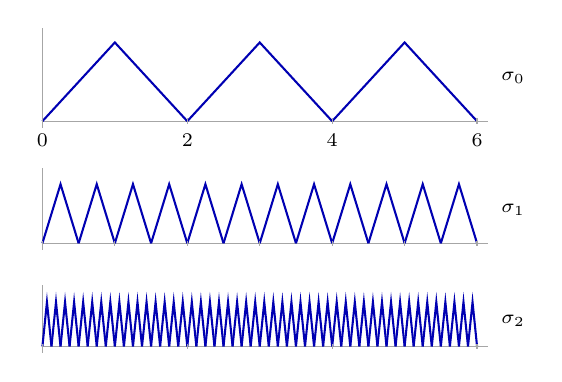
\begin{tikzpicture}[
  x=0.92cm,
  y=1.0cm,
  every node/.style={font=\scriptsize},
  axis/.style={gray!70, line width=0.45pt},
  wave/.style={blue!70!black, line width=0.75pt}
]
  % sigma_0 row
  \draw[axis] (0,0) -- (6.15,0);
  \draw[axis] (0,-0.08) -- (0,1.18);
  \foreach \i in {0,1,2} {
    \pgfmathsetmacro{\a}{2*\i}
    \pgfmathsetmacro{\b}{\a+1}
    \pgfmathsetmacro{\c}{\a+2}
    \draw[wave] (\a,0) -- (\b,1) -- (\c,0);
  }
  \foreach \x in {0,2,4,6} {
    \draw[axis] (\x,0.04) -- (\x,-0.04);
    \node[below] at (\x,-0.04) {$\x$};
  }
  \node[right] at (6.2,0.55) {$\sigma_0$};

  % sigma_1 row
  \begin{scope}[yshift=-1.55cm]
    \draw[axis] (0,0) -- (6.15,0);
    \draw[axis] (0,-0.08) -- (0,0.95);
    \foreach \i in {0,...,11} {
      \pgfmathsetmacro{\a}{0.5*\i}
      \pgfmathsetmacro{\b}{\a+0.25}
      \pgfmathsetmacro{\c}{\a+0.5}
      \draw[wave] (\a,0) -- (\b,0.75) -- (\c,0);
    }
    \foreach \x in {0,1,2,3,4,5,6} {
      \draw[axis] (\x,0.035) -- (\x,-0.035);
    }
    \node[right] at (6.2,0.42) {$\sigma_1$};
  \end{scope}

  % sigma_2 row
  \begin{scope}[yshift=-2.86cm]
    \draw[axis] (0,0) -- (6.15,0);
    \draw[axis] (0,-0.08) -- (0,0.78);
    \foreach \i in {0,...,47} {
      \pgfmathsetmacro{\a}{0.125*\i}
      \pgfmathsetmacro{\b}{\a+0.0625}
      \pgfmathsetmacro{\c}{\a+0.125}
      \draw[wave] (\a,0) -- (\b,0.5625) -- (\c,0);
    }
    \foreach \x in {0,2,4,6} {
      \draw[axis] (\x,0.03) -- (\x,-0.03);
    }
    \node[right] at (6.2,0.32) {$\sigma_2$};
  \end{scope}
\end{tikzpicture}

  \caption{The first compressed sawtooth terms $\sigma_k(x)=(3/4)^k\varphi(4^kx)$: heights shrink, slopes grow.}
  \label{fig:takagi-sawtooth-building-block}
\end{figure}

\begin{perspective} \label{per:nowhere-differentiability-explicit-and-generic} \hlt{Explicit Versus Generic Pathology}\\
The sawtooth series proves existence; Baire category shows nowhere differentiability is residual in $C([a,b],\R)$.
\end{perspective}

\begin{theorem} \label{thm:differentiable-somewhere-first-category} \hlt{Generic Nowhere Differentiability on Compact Intervals}\\
Let $a<b$, and let $C=C([a,b],\R)$ with the supremum metric. There exists a residual set $\mathcal{G}\subseteq C$ such that:
\begin{enumerate}[label=(\roman*)]
\setlength{\itemsep}{0pt}
\item no $f\in\mathcal{G}$ has an available one-sided derivative at any point of $[a,b]$;
\item no $f\in\mathcal{G}$ is monotone on any nondegenerate subinterval of $[a,b]$;
\item the set $\{f\in C:f\text{ is differentiable at some point of }[a,b]\}$ is first category.
\end{enumerate}
\begin{proof}
\begin{enumerate}[label=(\roman*)]
\setlength{\itemsep}{0pt}
\item Write $\Delta_hf(x)\defeq f(x+h)-f(x)$, and choose $N_0$ with $1/N_0<b-a$. For $n\geq N_0$, define
\begin{align}
R_n&\defeq\left\{f\in C:\forall x\in[a,b-1/n]\ \exists h>0\text{ with }\left|\frac{\Delta_hf(x)}{h}\right|>n\right\}, \nonumber\\
L_n&\defeq\left\{f\in C:\forall x\in[a+1/n,b]\ \exists h<0\text{ with }\left|\frac{\Delta_hf(x)}{h}\right|>n\right\}, \nonumber\\
G_n&\defeq\{f\in C:f\text{ is nonmonotone on every subinterval of length }1/n\}. \nonumber
\end{align}
Each $R_n,L_n,G_n$ is open and dense in $C$ (Weierstrass Approximation Theorem \ref{thm:weierstrass-polynomial-approximation}), plus small high-slope sawtooth perturbation; openness follows from compactness and uniform perturbation estimates.
\item Set $\mathcal{G}\defeq\bigcap_{n\geq N_0}(R_n\cap L_n\cap G_n)$. By Definition \ref{def:residual-thick-generic-set}, $\mathcal{G}$ is residual. If $f\in\mathcal{G}$, then the $R_n$ and $L_n$ conditions give one-sided difference quotients of arbitrarily large absolute value; since $f$ is bounded, the corresponding increments tend to $0$. Thus no available one-sided derivative exists.
\item Let $f\in\mathcal{G}$. Every nondegenerate subinterval contains a subinterval of length $1/n$ for all sufficiently large $n$, so the $G_n$ conditions make $f$ nonmonotone on every nondegenerate subinterval. If $f$ is differentiable somewhere, then $f\notin\mathcal{G}$; hence the differentiable-somewhere set lies in $C\setminus\mathcal{G}$, which is first category.
\end{enumerate}
\hlt{Structural Commentary}: Baire category turns dense sawtooth perturbability into a generic regularity failure.\\
\hlt{Key Insight}: The explicit construction shows existence; the category proof shows typicality.
\end{proof}
\end{theorem}

\begin{method} \label{meth:power-approx-fourier-proof-patterns-source-todo}\label{meth:power-series-approximation-proof-patterns} \hlt{Power-Series and Approximation Proof Patterns}
\begin{enumerate}[label=(\roman*)]
\setlength{\itemsep}{0pt}
\item \hlt{Power series}: work on $K_\rho\Subset I_R$; use uniform convergence before termwise limits or derivatives.
\item \hlt{Endpoint theorems}: prove identities inside the radius and pass to endpoints with Abel-type control.
\item \hlt{Approximate identities}: use kernels $Q_n\geq0$, $\int Q_n=1$, with tails $\to0$ off $0$.
\item \hlt{Uniform closure}: show $a_n\in\mathcal{A}$ and $a_n\rightrightarrows f$.
\item \hlt{Lattice closure}: derive $\abs{f}$, then $\max,\min$ from algebraic formulas.
\item \hlt{Stone--Weierstrass}: interpolate locally; use compactness and finite max/min to globalize.
\end{enumerate}
\hlt{Key Insight}: Uniform convergence and compactness are what make infinite algebra behave like finite algebra.
\end{method}
